\documentclass[letterpaper]{article}
\usepackage[margin=1in]{geometry}
\usepackage[utf8]{inputenc}
\usepackage{textcomp}
\usepackage{amssymb}
\usepackage{natbib}
\usepackage{graphicx}
\usepackage{gensymb}
\usepackage{amsthm, amsmath, mathtools}
\usepackage[dvipsnames]{xcolor}
\usepackage{enumerate}
\usepackage{mdframed}
\usepackage[most]{tcolorbox}
\usepackage{csquotes}
% https://tex.stackexchange.com/questions/13506/how-to-continue-the-framed-text-box-on-multiple-pages

\tcbuselibrary{theorems}

\newcommand{\R}{\mathbb{R}}
\newcommand{\Z}{\mathbb{Z}}
\newcommand{\N}{\mathbb{N}}
\newcommand{\Q}{\mathbb{Q}}
\newcommand{\C}{\mathbb{C}}
\newcommand{\code}[1]{\texttt{#1}}
\newcommand{\mdiamond}{$\diamondsuit$}
\newcommand{\PowerSet}{\mathcal{P}}
\newcommand{\Mod}[1]{\ (\mathrm{mod}\ #1)}
\DeclareMathOperator{\lcm}{lcm}

%\newtheorem*{theorem}{Theorem}
%\newtheorem*{definition}{Definition}
%\newtheorem*{corollary}{Corollary}
%\newtheorem*{lemma}{Lemma}
\newtheorem*{proposition}{Proposition}


\newtcbtheorem[number within=section]{theorem}{Theorem}
{colback=green!5,colframe=green!35!black,fonttitle=\bfseries}{th}

\newtcbtheorem[number within=section]{definition}{Definition}
{colback=blue!5,colframe=blue!35!black,fonttitle=\bfseries}{def}

\newtcbtheorem[number within=section]{corollary}{Corollary}
{colback=yellow!5,colframe=yellow!35!black,fonttitle=\bfseries}{cor}

\newtcbtheorem[number within=section]{lemma}{Lemma}
{colback=red!5,colframe=red!35!black,fonttitle=\bfseries}{lem}

\newtcbtheorem[number within=section]{example}{Example}
{colback=white!5,colframe=white!35!black,fonttitle=\bfseries}{def}

\newtcbtheorem[number within=section]{note}{Important Note}{
        enhanced,
        sharp corners,
        attach boxed title to top left={
            xshift=-1mm,
            yshift=-5mm,
            yshifttext=-1mm
        },
        top=1.5em,
        colback=white,
        colframe=black,
        fonttitle=\bfseries,
        boxed title style={
            sharp corners,
            size=small,
            colback=red!75!black,
            colframe=red!75!black,
        } 
    }{impnote}
\usepackage[utf8]{inputenc}
\usepackage[english]{babel}
\usepackage{fancyhdr}
\usepackage[hidelinks]{hyperref}
\usepackage{csquotes}

\pagestyle{fancy}
\fancyhf{}
\rhead{Math 187A}
\chead{Monday, February 06, 2023}
\lhead{Lecture 12}
\rfoot{\thepage}

\setlength{\parindent}{0pt}

\begin{document}

\section{Classical \& Modified Gram-Schmidt}
In this lecture, we'll talk about the classical and modified Gram-Schmidt algorithms. 

\subsection{Classical Algorithm}
Given $A$, we want to find $\hat{Q}$ and $\hat{R}$ such that 
\begin{equation}{\label{2-6:1}}
    A = \hat{Q}\hat{R}.
\end{equation} Note that we can rewrite ({\ref{2-6:1}}) in the form 
\[\begin{bmatrix}
    a_1 & a_2 & \hdots & a_m
\end{bmatrix} = \begin{bmatrix}
    q_1 & q_2 & \hdots & q_m
\end{bmatrix} \begin{bmatrix}
    r_{11} & r_{12} & \hdots & r_{1m} \\ 
    0      & r_{22} & \hdots & r_{2m} \\ 
    \vdots & \vdots & \ddots & \vdots \\ 
    0      & 0      & 0      & r_{mm} 
\end{bmatrix}.\] 
The formula to finding these entries are 
\[a_m = q_1 r_{1m} + q_2 r_{2m} + \hdots + q_m r_{mm}.\]
\[r_{ji} = \begin{cases}
    \cyclic{a_{i}, q_{j}} & j < i \\ 
    \left|\left| a_i - \sum_{k = 1}^{i - 1} r_{ki} q_k \right|\right|_2 & j = i \\ 
    0 & j > i
\end{cases}.\]
\[q_{i} = \frac{a_i - \sum_{j = 1}^{i - 1} r_{ji} q_j}{r_{ii}}.\]
$a_i$ is a vector and $r_{ij}$ is a scalar. 

\subsubsection{Worked Example}
\begin{mdframed}
    (Example.) Suppose we have \[A = \begin{bmatrix}
        -1 & -1 & 1 \\ 
        1 & 3 & 3 \\ 
        -1 & -1 & 5 \\ 
        1 & 3 & 7
    \end{bmatrix}.\]
    We can define 
    \[\vec{a_1} = \begin{bmatrix}
        -1 \\ 1 \\ -1 \\ 1
    \end{bmatrix} \quad \vec{a_2} = \begin{bmatrix}
        -1 \\ 3 \\ -1 \\ 3
    \end{bmatrix} \quad \vec{a_3} = \begin{bmatrix}
        1 \\ 3 \\ 5 \\ 7
    \end{bmatrix}.\]
    In other words, our goal is to get something like 
    \[A = \begin{bmatrix}
        a_1 & a_2 & a_3
    \end{bmatrix} = \begin{bmatrix}
        q_1 & q_2 & q_3
    \end{bmatrix} \begin{bmatrix}
        r_{11} & r_{12} & r_{13} \\ 
        0 & r_{22} & r_{23} \\ 
        0 & 0 & r_{33}
    \end{bmatrix}.\]
    Then, we can find the elements of $\hat{Q}$ and $\hat{R}$. 
    \begin{mdframed}
        \[a_1 = q_1 r_{11} \implies q_1 = \frac{a_1}{r_{11}}.\]
        Since $q_1$ is a unit vector (remember that the $q_i$'s are in an orthonormal set), it follows that $||q_1||_2 = 1$. Then, 
        \[r_{11} = ||a_{1}||_2 = \sqrt{(-1)^2 + 1^2 + (-1)^2 + 1^2} = 2.\]
        Notice that 
        \[q_1 = \frac{a_1}{2} = \frac{1}{2} \begin{bmatrix}
            -1 \\ 1 \\ -1 \\ 1 
        \end{bmatrix} = \begin{bmatrix}
            -\frac{1}{2} \\ \frac{1}{2} \\ -\frac{1}{2} \\ \frac{1}{2}
        \end{bmatrix}.\]
    \end{mdframed}

    \begin{mdframed}
        \[a_2 = q_1 r_{12} + q_2 r_{22}.\]
        Because $q_1$ and $q_2$ are orthonormal, we know that $\cyclic{q_2, q_2} = 1$ and $\cyclic{q_1, q_2} = 0$. So, \[\cyclic{a_2, q_1} = \cyclic{q_1 r_{12} + q_2 r_{22}, q_1} = r_{12} \underbrace{\cyclic{q_1, q_1}}_{1} + r_{22} \underbrace{\cyclic{q_2, q_1}}_{0} = r_{12}\]
        Then, 
        \begin{equation*}
            \begin{aligned}
                r_{12} &= \cyclic{a_{2}, q_{1}}= \begin{bmatrix}
                        -1 & 3 & -1 & 3
                    \end{bmatrix} \begin{bmatrix}
                        -\frac{1}{2} \\ \frac{1}{2} \\ -\frac{1}{2} \\ \frac{1}{2}
                    \end{bmatrix} \\ 
                    &= (-1) \left(-\frac{1}{2}\right) + (3) \left(\frac{1}{2}\right) + (-1)\left(-\frac{1}{2}\right) + (3)\left(\frac{1}{2}\right) \\ 
                    &= 4.
            \end{aligned}
        \end{equation*}
        Now, we need to find 
        \[q_2 = \frac{a_2 - \sum_{j = 1}^{1} r_{ji}q_j}{r_{22}}.\]
        \begin{itemize}
            \item Note that 
            \begin{equation*}
                \begin{aligned}
                    r_{22} &= \left|\left| a_2 - \sum_{k = 1}^{1} r_{k2} q_k \right|\right|_2 = \left|\left| a_2 - r_{12} q_1 \right|\right|_2 \\ 
                        &= \left|\left| \begin{bmatrix}
                            -1 \\ 3 \\ -1 \\ 3
                        \end{bmatrix} - 4 \begin{bmatrix}
                            -\frac{1}{2} \\ \frac{1}{2} \\ -\frac{1}{2} \\ \frac{1}{2}
                        \end{bmatrix} \right|\right|_2 = \left|\left| \begin{bmatrix}
                            -1 \\ 3 \\ -1 \\ 3
                        \end{bmatrix} - \begin{bmatrix}
                            -2 \\ 2 \\ -2 \\ 2
                        \end{bmatrix} \right|\right|_2 \\ 
                        &= \left|\left| \begin{bmatrix}
                            1 \\ 1 \\ 1 \\ 1
                        \end{bmatrix} \right|\right|_2 = \sqrt{1^2 + 1^2 + 1^2 + 1^2} = \sqrt{4} = 2.
                \end{aligned}
            \end{equation*}
            \item From this, it follows that 
            \[q_2 = \frac{a_2 - r_{12} q_1}{r_{22}} = \frac{1}{r_{22}}(a_2 - r_{12} q_1) = \frac{1}{2}\left(\begin{bmatrix}
                -1 \\ 3 \\ -1 \\ 3
            \end{bmatrix} - 4 \begin{bmatrix}
                -\frac{1}{2} \\ \frac{1}{2} \\ -\frac{1}{2} \\ \frac{1}{2}
            \end{bmatrix}\right) = \frac{1}{2}\begin{bmatrix}
                1 \\ 1 \\ 1 \\ 1
            \end{bmatrix} = \begin{bmatrix}
                \frac{1}{2} \\ \frac{1}{2} \\ \frac{1}{2} \\ \frac{1}{2}
            \end{bmatrix}.\]
        \end{itemize}
    \end{mdframed}

    \begin{mdframed}
        \[a_3 = r_{13} q_1 + r_{23}q_2 + r_{33}q_3.\]
        At this point, we know that 
        \[q_1 = \begin{bmatrix}
            -\frac{1}{2} \\ \frac{1}{2} \\ -\frac{1}{2} \\ \frac{1}{2}
        \end{bmatrix} \quad q_2 = \begin{bmatrix}
            \frac{1}{2} \\ \frac{1}{2} \\ \frac{1}{2} \\ \frac{1}{2}
        \end{bmatrix} \quad a_3 = \begin{bmatrix}
            1 \\ 3 \\ 5 \\ 7
        \end{bmatrix}.\]
        Additionally, $\cyclic{q_1, q_3} = \cyclic{q_2, q_3} = 0$ while $\cyclic{q_3, q_3} = 1$. From there, we have
        \[r_{13} = \cyclic{a_3, q_1} = \begin{bmatrix}
            1 & 3 & 5 & 7
        \end{bmatrix} \begin{bmatrix}
            -\frac{1}{2} \\ \frac{1}{2} \\ -\frac{1}{2} \\ \frac{1}{2}
        \end{bmatrix} = 1\left(-\frac{1}{2}\right) + 3\left(\frac{1}{2}\right) + 5\left(-\frac{1}{2}\right) + 7\left(\frac{1}{2}\right) = 2\]
        and 
        \[r_{23} = \cyclic{a_3, q_2} = \begin{bmatrix}
            1 & 3 & 5 & 7
        \end{bmatrix} \begin{bmatrix}
            \frac{1}{2} \\ \frac{1}{2} \\ \frac{1}{2} \\ \frac{1}{2}
        \end{bmatrix} = 8\]
        and 
        \begin{equation*}
            \begin{aligned}
                r_{33} &= \left|\left| a_3 - \sum_{k = 1}^{2} r_{k3} q_k \right|\right|_2 \\ 
                    &= \left|\left| a_3 - (r_{13} q_1 + r_{23} q_2) \right|\right|_2 \\ 
                    &= \left|\left| \begin{bmatrix}
                        1 \\ 3 \\ 5 \\ 7
                    \end{bmatrix} - \left(2 \begin{bmatrix}
                        -\frac{1}{2} \\ \frac{1}{2} \\ -\frac{1}{2} \\ \frac{1}{2}
                    \end{bmatrix} + 8 \begin{bmatrix}
                        \frac{1}{2} \\ \frac{1}{2} \\ \frac{1}{2} \\ \frac{1}{2}
                    \end{bmatrix}\right) \right|\right|_2 \\ 
                    &= \left|\left| \begin{bmatrix}
                        -2 \\ -2 \\ 2 \\ 2
                    \end{bmatrix} \right|\right|_2 \\ 
                    &= \sqrt{(-2)^2 + (-2)^2 + 2^2 + 2^2} \\ 
                    &= \sqrt{4 + 4 + 4 + 4} \\ 
                    &= 4.
            \end{aligned}
        \end{equation*}
        Finally,
        \begin{equation*}
            \begin{aligned}
                q_3 &= \frac{a_3 - \sum_{j = 1}^{2} r_{j3}q_j}{r_{33}} = \frac{a_3 - (r_{13}q_1 + r_{23}q_2)}{r_{33}} = \frac{1}{r_{33}} (a_3 - (r_{13}q_1 + r_{23}q_2)) \\ 
                    &= \frac{1}{4} \begin{bmatrix}
                        -2 \\ -2 \\ 2 \\ 2
                    \end{bmatrix} = \begin{bmatrix}
                        -\frac{1}{2} \\ -\frac{1}{2} \\ \frac{1}{2} \\ \frac{1}{2}
                    \end{bmatrix}.
            \end{aligned}
        \end{equation*}
    \end{mdframed}

    Notice that we're now done with the algorithm. In particular, we have 
    \[q_1 = \begin{bmatrix}
        -\frac{1}{2} \\ \frac{1}{2} \\ -\frac{1}{2} \\ \frac{1}{2}
    \end{bmatrix} \quad q_2 = \begin{bmatrix}
        \frac{1}{2} \\ \frac{1}{2} \\ \frac{1}{2} \\ \frac{1}{2}
    \end{bmatrix} \quad q_3 = \begin{bmatrix}
        -\frac{1}{2} \\ -\frac{1}{2} \\ \frac{1}{2} \\ \frac{1}{2}
    \end{bmatrix},\]
    and 
    \[r_{11} = 2 \quad r_{12} = 4 \quad r_{13} = 2 \quad r_{22} = 2 \quad r_{23} = 8 \quad r_{33} = 4.\]
    This gives us the decomposition of 
    \[\underbrace{\begin{bmatrix}
        -1 & -1 & 1 \\ 
        1 & 3 & 3 \\ 
        -1 & -1 & 5 \\ 
        1 & 3 & 7
    \end{bmatrix}}_{A} = \underbrace{\begin{bmatrix}
        -\frac{1}{2} & \frac{1}{2} & -\frac{1}{2} \\ 
        \frac{1}{2} & \frac{1}{2} & -\frac{1}{2} \\ 
        -\frac{1}{2} & \frac{1}{2} & \frac{1}{2} \\ 
        \frac{1}{2} & \frac{1}{2} & \frac{1}{2}
    \end{bmatrix}}_{\hat{Q}} \underbrace{\begin{bmatrix}
        2 & 4 & 2 \\ 
        0 & 2 & 8 \\ 
        0 & 0 & 4
    \end{bmatrix}}_{\hat{R}}.\]
\end{mdframed}

\subsubsection{Summary}
This is effectively how the \textbf{classical Gram-Schmidt} algorithm works. Notice how we went through each $\vec{a_i}$ entry (column by column) and found all the desired values of $\vec{q_i}$ and $r_{ij}$. 

\bigskip 

Sadly, the classical Gram-Schmidt is \textbf{unstable}\footnote{A very small change of some entry in $A$ can yield a significant difference in the resulting $QR$ decomposition.}. For this reason, we'll introduce a \emph{modified} Gram-Schmidt algorithm, which is \textbf{stable}. One notable difference is that 
\begin{itemize}
    \item The classical algorithm builds $R$ one \emph{column} at a time. 
    \item The modified algorithm builds $R$ one \emph{row} at a time.
\end{itemize}
\begin{center}
    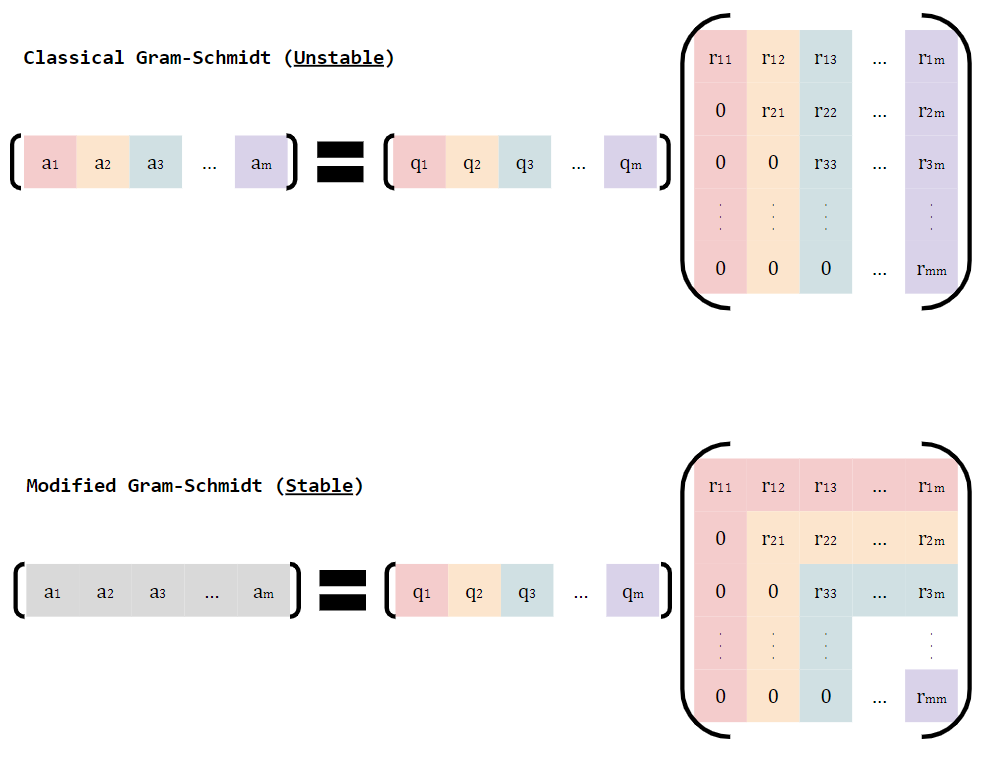
\includegraphics[scale=0.75]{../assets/gram.png}
\end{center}

\subsubsection{MATLAB Code}
\begin{mdframed}
    \begin{verbatim}
function [Q,R]=classicalGS(A)         % classical Gram-Schmidt

n = size(A,2);                        % number of columns; this formulation
                                      % does not need the number of rows
for i=1:n                             
Q(:,i) = A(:,i);                      % initialization
   
    for j=1:(i-1)
        R(j,i)=(A(:,i))'*Q(:,j);      % computing R(j,i) by going down the column
        Q(:,i)=Q(:,i)-R(j,i)*Q(:,j);  % updating Q(:,j)
    end
   
    R(i,i) = norm(Q(:,i));            % computing R(i,i) 
    Q(:,i)=Q(:,i)/R(i,i);             % making Q(:,i) a unit vector
end
    \end{verbatim}
\end{mdframed}


\subsection{Modified Gram-Schmidt}
As mentioned earlier, the modified Gram-Schmidt is a stable algorithm that builds $R$ one row at a time. 

\subsubsection{MATLAB Code}
\begin{mdframed}
    \begin{verbatim}
function [Q,R]=modifiedGS(A)          % modified Gram-Schmidt

n = size(A,2);                        % number of columns; this formulation
                                      % does not need the number of rows
for i=1:n                             
    Q(:,i) = A(:,i);                  % initialization
end

for i=1:n
    R(i,i) = norm(Q(:,i));            % computing R(i,i) 
    Q(:,i)=Q(:,i)/R(i,i);             % making Q(:,i) a unit vector

    for j=(i+1):n
        R(i,j)=(Q(:,i))'*Q(:,j);      % computing R(i,j) by going right on ith row
        Q(:,j)=Q(:,j)-R(i,j)*Q(:,i);  % updating Q(:,j)
    end

end
    \end{verbatim}
\end{mdframed}

\subsubsection{Worked Example}
We'll base our algorithm on the MATLAB code above. 
\begin{mdframed}
    (Example.) We'll solve the same problem as in the previous example, \emph{except} we'll use the modified algorithm instead. To reiterate, suppose we have \[A = \begin{bmatrix}
        -1 & -1 & 1 \\ 
        1 & 3 & 3 \\ 
        -1 & -1 & 5 \\ 
        1 & 3 & 7
    \end{bmatrix}.\]
    We can define 
    \[\vec{a_1} = \begin{bmatrix}
        -1 \\ 1 \\ -1 \\ 1
    \end{bmatrix} \quad \vec{a_2} = \begin{bmatrix}
        -1 \\ 3 \\ -1 \\ 3
    \end{bmatrix} \quad \vec{a_3} = \begin{bmatrix}
        1 \\ 3 \\ 5 \\ 7
    \end{bmatrix}.\]
    In other words, our goal is to get something like 
    \[A = \begin{bmatrix}
        a_1 & a_2 & a_3
    \end{bmatrix} = \begin{bmatrix}
        q_1 & q_2 & q_3
    \end{bmatrix} \begin{bmatrix}
        r_{11} & r_{12} & r_{13} \\ 
        0 & r_{22} & r_{23} \\ 
        0 & 0 & r_{33}
    \end{bmatrix}.\]
    \textbf{Keep this in mind}, since we'll be assuming this. Then, we can find the elements of $\hat{Q}$ and $\hat{R}$. We'll run through the algorithm described in code above. 
    \begin{enumerate}
        \item First, we define $q_1 = a_1$, $q_2 = a_2$, and $q_3 = a_3$. 
        
        \item Next, for we want to find $r_{11}$, $r_{12}$, $r_{13}$ and then determine $q_1$. We can also update $q_2$ and $q_3$. 
        
        \begin{itemize}
            \item (Outer Loop: $i = 1$.) Note that 
            \[r_{11} = ||q_1||_2 = ||a_1||_2 = \sqrt{(-1)^2 + 1^2 + (-1)^2 + 1^2} = 2.\]
            Here, $r_{11} = ||q_1||_2$ comes from the algorithm (since we \emph{initially} set $q_1 = a_1$.)
            \[q_1 = \frac{q_1}{r_{11}} = \frac{q_1}{||a_1||_2} = \begin{bmatrix}
                -1/2 \\ 1/2 \\ -1/2 \\ 1/2
            \end{bmatrix}.\]
            Here, we've updated the value of $q_1$. 
    
            \item In the \emph{inner loop}, we do the following for $j = 2$ to $3$:
            \begin{itemize}
                \item (Inner Loop: $j = 2$.) Next, note that 
                \[r_{12} = \cyclic{q_1, q_2} = q_1^T q_2 = q_1^T a_2 = \left(-\frac{1}{2}\right)(-1) + \frac{1}{2}(3) + \left(-\frac{1}{2}\right)(-1) + \frac{1}{2}(3) = 4.\]
                From there, it follows that 
                \[q_2 = q_2 - r_{12}q_1 = \begin{bmatrix}
                    -1 \\ 3 \\ -1 \\ 3
                \end{bmatrix} - 4 \begin{bmatrix}
                    -1/2 \\ 1/2 \\ -1/2 \\ 1/2
                \end{bmatrix} = \begin{bmatrix}
                    1 \\ 1 \\ 1 \\ 1
                \end{bmatrix}.\]
        
                \item (Inner Loop: $j = 3$.) Next, we have 
                \[r_{13} = \cyclic{q_1, q_3} = q_1^T q_3 = q_1^T a_3 = \left(-\frac{1}{2}\right)(1) + \frac{1}{2}(3) + \left(-\frac{1}{2}\right)(5) + \frac{1}{2}7 = 2.\]
                From there, it follows that 
                \[q_3 = q_3 - r_{13}q_1 = \begin{bmatrix}
                    1\\3\\5\\7
                \end{bmatrix} - 2\begin{bmatrix}
                    -1/2 \\ 1/2 \\ -1/2 \\ 1/2
                \end{bmatrix} = \begin{bmatrix}
                    2 \\ 2 \\ 6 \\ 6
                \end{bmatrix}.\]
            \end{itemize}
        \end{itemize}
        
        \item After running through the first iteration of the outer loop discussed in the algorithm, we have 
        \[q_2 = \begin{bmatrix}
            1\\1\\1\\1
        \end{bmatrix} \quad q_3 = \begin{bmatrix}
            2\\2\\6\\6
        \end{bmatrix}.\] 
        Now, we want to find $r_{22}$, $r_{23}$, and determine $q_2$. We also update $q_3$. 
        \begin{itemize}
            \item (Outer Loop: $i = 2$.) We have 
            \[r_{22} = ||q_2||_2 = \sqrt{1^2 + 1^2 + 1^2 + 1^2} = 2.\]
            So, updating $q_2$ gives us 
            \[q_2 = \frac{q_2}{r_{22}} = \begin{bmatrix}
                1/2 \\ 1/2 \\ 1/2 \\ 1/2
            \end{bmatrix}.\] 

            \item In the \emph{inner loop}, we do the following for $j = 3$ to $3$:
            \begin{itemize}
                \item (Inner Loop: $j = 3$.) We have 
                \[r_{23} = \cyclic{q_2, q_3} = q_2^T = q_3 = \frac{1}{2}(2) + \frac{1}{2}(2) + \frac{1}{2}(6) + \frac{1}{2}(6) = 8.\]
                From there, 
                \[q_3 = q_3 - r_{23}q_2 = \begin{bmatrix}
                    2\\2\\6\\6
                \end{bmatrix} - 8\begin{bmatrix}
                    1/2 \\ 1/2 \\ 1/2 \\ 1/2
                \end{bmatrix} = \begin{bmatrix}
                    -2 \\ -2 \\ 2 \\ 2
                \end{bmatrix}.\]
            \end{itemize}
        \end{itemize}

        \item After running through the second iteration of the outer loop discussed in the algorithm, we have 
        \[q_3 = \begin{bmatrix}
            -2 \\ -2 \\ 2 \\ 2
        \end{bmatrix}.\]
        Now, we can find $r_{33}$ and determine the value of $q_3$. 
        \begin{itemize}
            \item (Outer Loop: $i = 3$.) We have 
            \[r_{33} = ||q_3||_2 = \sqrt{(-2)^2 + (-2)^2 + 2^2 + 2^2} = 4.\]
            So, 
            \[q_3 = \frac{q_3}{r_{33}} = \begin{bmatrix}
                -1/2 \\ -1/2 \\ 1/2 \\ 1/2
            \end{bmatrix}.\]

            \item Notice that the inner loop is not executed since $j = 4$ is greater than $3$.
        \end{itemize}
    \end{enumerate}
\end{mdframed}


\end{document}